\chapter{Data Discussion and Policy Construction}\label{C:us}

In this section I discuss the construction of my reputation policies for use on Twitter. In particular the development of analysis tools for achieving greater understanding of the Twitter dataset created will be discussed, and discussion of hypotheses generated from this data and how we experimented with these. %Fix this

\section{Social Media Selection}

Until now, the reasoning behind my social media selection has been largely neglected. In order to gather useful data, I looked at the various social media sites in the context of gathering reputation data, and seeing what could be fetched. %Add to this. Not very good currently... 

In order to scrape useful information, I needed to look at the various social media sites in the context of gathering reputation data, and seeing what could be selected. 

\begin{itemize}

\item Facebook: Publicly available information on Facebook includes data such as a user's Likes, Posts to Walls, and Friend networks. 
\item LinkedIn: The primary business social network on which professionals can display information pertaining to their career and skills. Reputation data is fairly concrete - endorsements, skills, groups, and recommendations. 
\item Twitter: The social networking site allowing posts of up to 140 characters. Information available is number of followers, number of profiles the person is following, number of posts, and post data itself. Post data includes retweet and favourite count, the content itself, as well as the people who retweeted the tweet itself. 
\item Google+: Google+ is similar to Facebook in style, and holds a large user base, but with much lower daily use than Facebook.
\item Slashdot: Slashdot is a social media and news network targeted at a 'geek' audience. Slashdot is one of few social media sites that uses a positive/negative rating system on posts. This inbuilt reputation system could be interesting to look at further, when porting data between social media platforms. It is also unique from the standpoint of identifying 'trolls' - for which the website is widely known. 
%\item  Facebook: As summarised above, much previous work has been done on looking at what information can be gathered from publicly available data on Facebook. Likes, Posts to Walls, and Friends are examples of data that is readily available on public profiles. Facebook has a difficulty with its strict and varying privacy settings, which is challenging in the context of a flexible scraper.
%\item LinkedIn: This is the primary business social network on which professionals can display information about their careers. Reputation data here is fairly concrete - LinkedIn carries the concept of endorsements on skills, as well as information on past roles and experience. 
%\item Twitter: Twitter is a social networking site allowing posts of up to 140 characters. This is another site with a decent market share - it is also more open to sharing than other sites. Twitter has an API that can be used to retrieve information from profiles, which should be more robust than web-scraping. There have been studies into behavioural analysis of twitter users, through the figures of number of followers, number following, and number of tweets. These three figures are publicly available. 
%\item Google+: Google+ is similar to Facebook in style, and holds a large user base, but with much lower daily users than Facebook. It poses similar challenges to Facebook due to its stricter privacy settings. Google is also known for its restrictive hand on web-scrapers. This makes retrieving data from Google+ an interesting exercise. 
\end{itemize}

\section{Retweet Analysis}

First present the use of retweets vs favourites on Twitter, and show that they are similar

Next we look at impact factor of a person's retweets, pulled from the Hirsch-index formula. 

Policies as an outcome of this, written using Ruler?

\begin{description}
 \item [H1.]{Retweet and Favourite use is equivalent on Twitter}
 \item [H2.]{Embedded social networks exist within Twitter, and can be detected. We predict that }
\end{description}

Our definition of equivalent defines that 

\section{Temporal Clustering}

\section{Community Detection}

\subsection{MapEquation}

This section discusses the design and implementation of my reputation policies associated with social media. 

There are lots of different areas to discuss. For example, temporal analysis, sentiment analysis, retweet/favourite analysis, community detection discussion. 

Constant emmitter - correlation between their impact factor and temporal bucketing will be higher than one-hit wonders. Detection for one-hit wonders. 

%Define the architectures that I considered for implementing web-scraper

%Option one - stand-alone web scraping libraries

%Option two - extend existing web scraper, utilise this.

\section{Policy Construction}

\section{Temporal}

\subsection{MapEquation}

Two phases to each facet of implementation; scraper, data understanding, and policy implementation and evaluation. Discuss each of these in seperate sections.

Define multiple hypotheses to add strength to the report

Brief description of LinkedIn Scraper. Ultimately decided that twitter had significant data interest to be the only focus of the project.

Discuss how the project was a study on what could be inferred from the data that we can access. Therefore some dead ends, etc. E.g. LinkedIn, Sentiment140 API for tweet analysis. 

Temporal analysis

Evaluation tool development

Phases of implementation for each tool. Design, implement scraper, implement data analysis components, implement evaluation components and policies. 

This section outlines my evaluation strategies, tests performed, and presents and discusses the results of evaluation conducted on the developed web scrapers. It then presents an evaluation of the policies and hypotheses formulated during analysis of data gathered. 

%Performance

%Resistance to Detection

%Logging



\section{Policy Evaluation}

This section outlines my evaluation strategies, tests performed, and presents and discusses the results of evaluation conduceted on the developed system. 

In order to evaluate my solution I need to refer back to the requirements gathered at the beginning of the project. 

- These requirements will be moved to the Requirements Analysis section... is just useful to have them stored here for easy referrals. 

\begin{itemize}
\item Develop a set of Policies that can be used to ...
\item Develop a metric of reliability of information gathered, based on privacy settings.
\item Potential to Develop an Interface with Filip Dimitrievski's project. Re-using my web-scraping libraries could be useful for his project. (Probably not going to happen)
\item Aggregate data for storage into GRAft
\end{itemize}

Non-Functional Requirements:
\begin{itemize}
\item Privacy Protection
\item Maintainability and Resistance to User-Interface Changes
\item Performance of Scrapers
\item Ability to Resist Blocking Detection, and Recover from Failure
\end{itemize}

\section{Policies}

\subsection{Correlation of Impact Factor vs Bucketed Impacts}

\begin{figure}[h!]
\centering
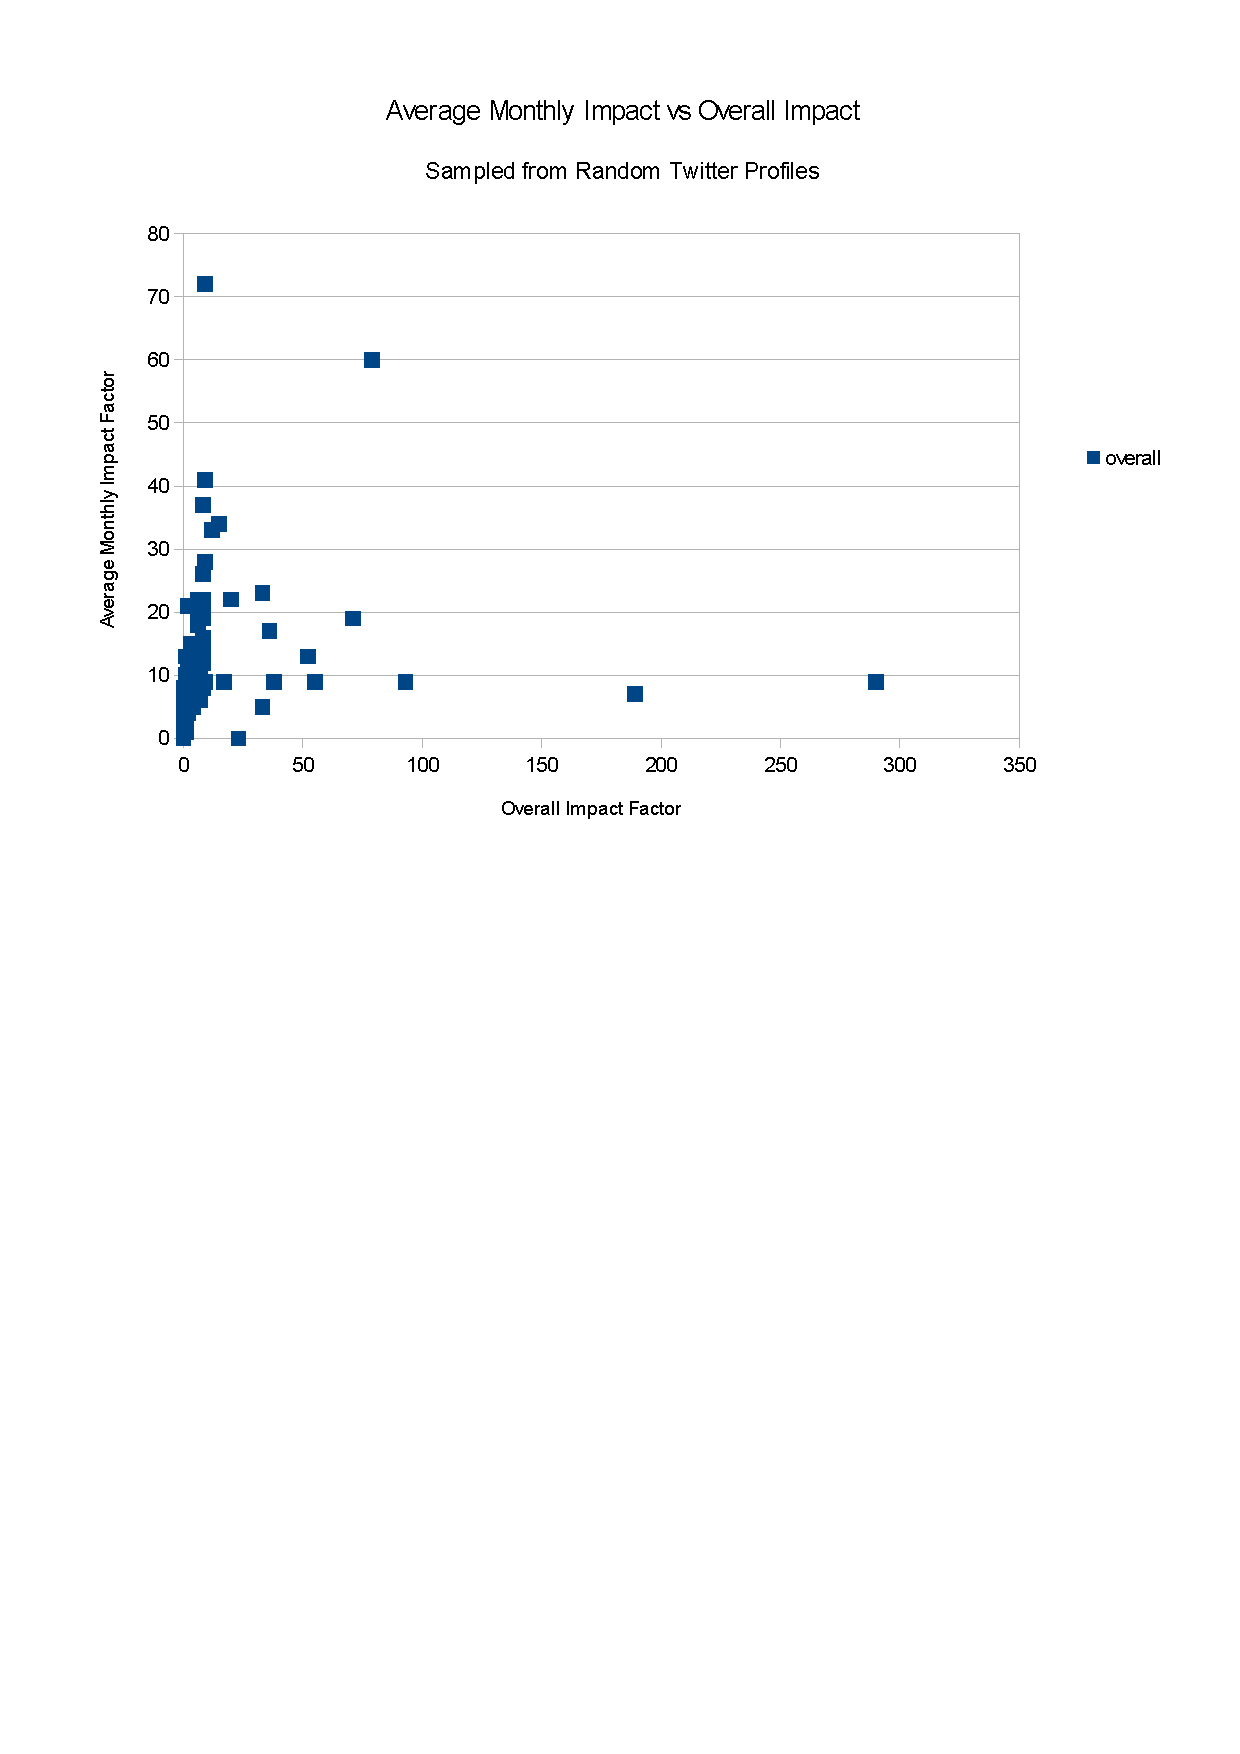
\includegraphics[width=400px]{Images/monthly_impact_vs_overallv2.pdf}
\caption{Monthly Impact against Overall Impact}
\end{figure}

\begin{figure}[h!]
\centering
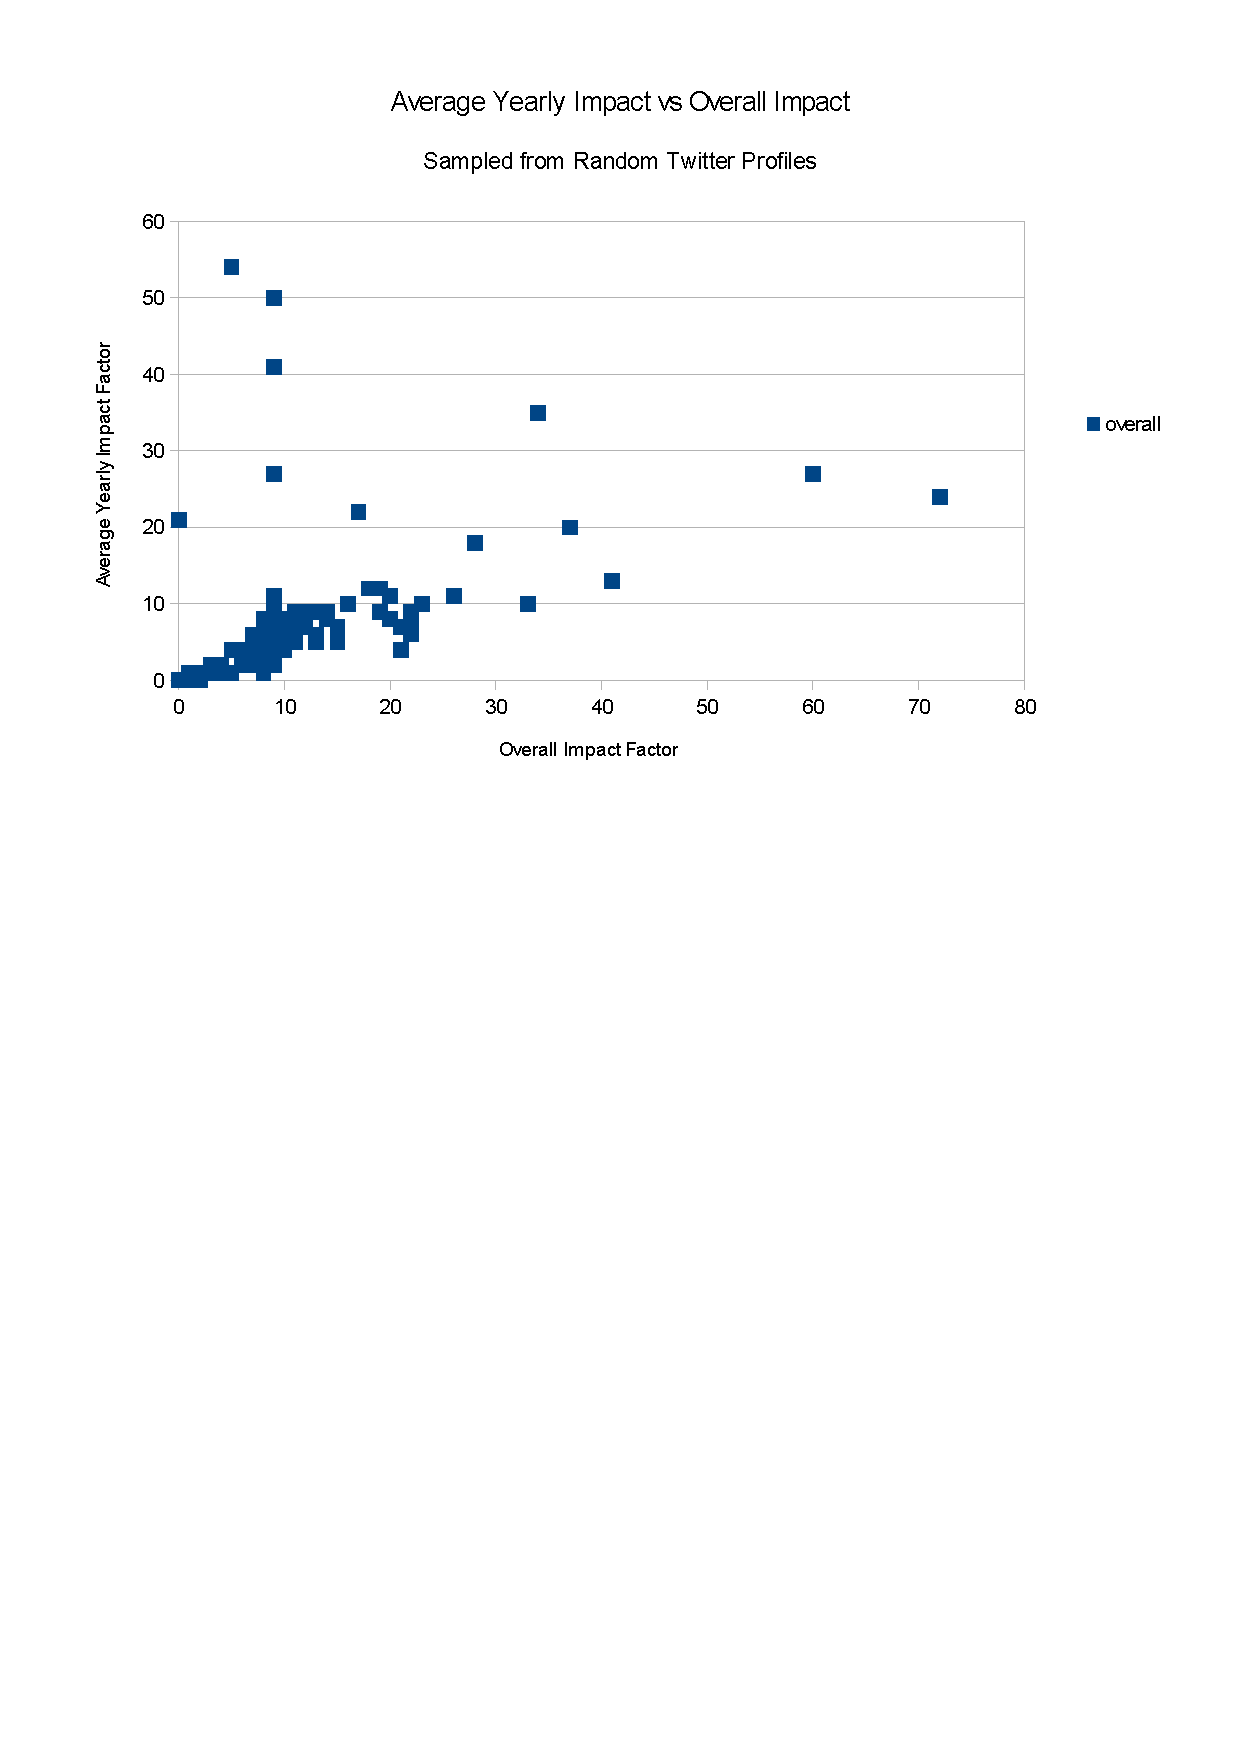
\includegraphics[width=400px]{Images/yearly_impact_vs_overallv2.pdf}
\caption{Yearly Impact against Overall Impact}
\end{figure}

One strategy for inferring reputation information that I looked at was through temporal bucketing of impact factor, into days, months, and years. The figures below show the relationship between people's mean monthly calculated impact factor (i.e. by calculating a person's impact score for each month, and then averaging these values over the total number of months), and the individual's overall impact score. I infer that there is a weak relationship between average monthly impact and overall impact (Pearson's correlation coefficient of 0.273(3 s.f.)), and a stronger relationship between average yearly impact and overall impact (r=0.689(3 s.f.))\\

\noindent What I believe this data shows is that the impact factor is favourable to individuals who are consistent on Twitter over time. 

\subsection{Results of Monthly Bucketing}

By applying the impact factor formula to individuals on a monthly basis, we are able to generate an impression of how regularly active a person is. The data also reveals how influential the person has been per month. This assists when comparing individuals who are consistently strongly influential (e.g. Barack Obama, companies such as instagram), with those who are popular for a limited period only. I looked at comparing different bucket sizes for this temporal aggregation. Days, months, and years were used as buckets, with monthly aggregation clearly showing the strongest and more interesting trends. 

\begin{figure}[h!]
\centering
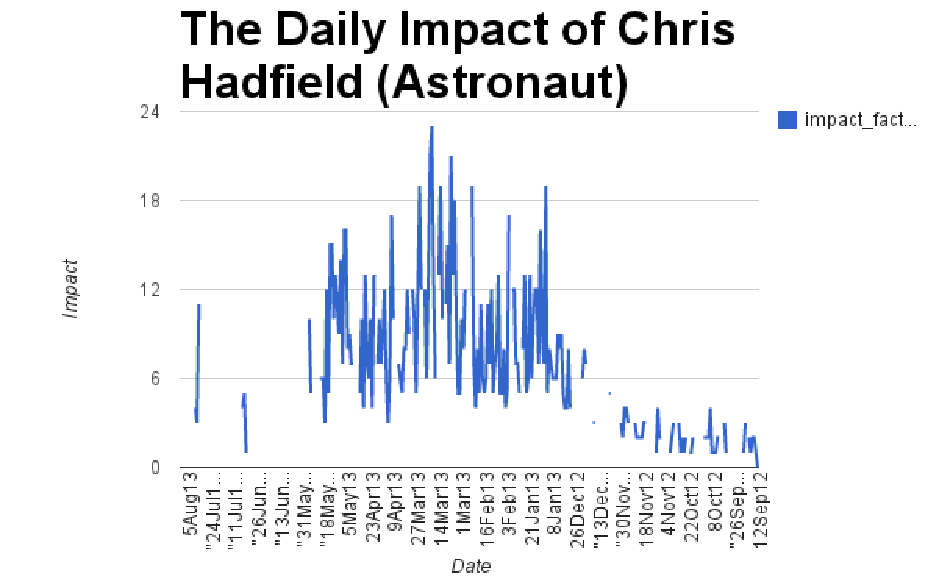
\includegraphics{Images/daily_impact_chris_hadfield.pdf}
\caption{The Daily Impact of Chris Hadfield - Famous Astronaut}
\end{figure}

\begin{figure}[h!]
\centering
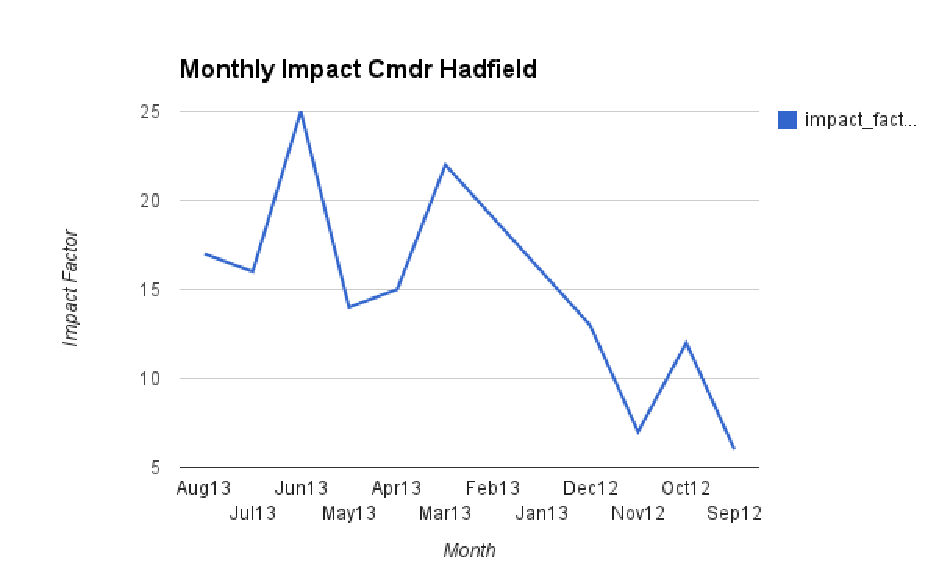
\includegraphics{Images/monthly_impact_chris_hadfield.pdf}
\caption{The Monthly Impact of Chris Hadfield - Famous Astronaut}
\end{figure}

\begin{figure}[h!]
\centering
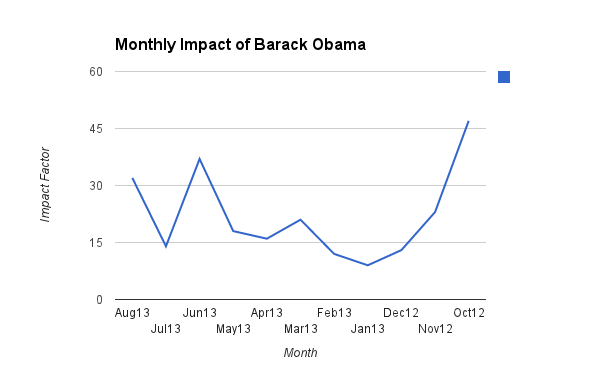
\includegraphics{Images/monthly_impact_barack_obama.png}
\caption{The Monthly Impact of Barack Obama - President of USA (As if you didn't know that)}
\end{figure}

We can see that the daily and monthly impact trends follow roughly the same curve, which should be expected. The difference is due to the strictness of the impact factor formula in classifying someone as 'influential'. It is very difficult to get a value much above 1 on a daily basis, unless you are very frequently both making use of the social media, and having people respond to this activity. 

\section{Scraper}

\subsection{Functional Requirements}

Aggregate data for storage into Graft - given that I am currently only storing data from Twitter this requirement has not yet been met.

Develop a metric of reliability of information gathered, based on privacy settings. Currently on Twitter there are two degrees of privacy - Open and Closed! Closed profiles means I cannot get any meaningful information, whereas on Open profiles I can get anything I want! Most profiles are open so this is not a concern. Profiles of celebrities etc are always set to open.

Developing a set of Policies - still in the production line, still experimenting with different ways of using the data.